\documentclass[12pt,a4paper,titlepage]{article}
\usepackage[utf8]{inputenc}
\usepackage[finnish]{babel}
\usepackage{setspace}
\usepackage{parskip}
\usepackage{amssymb}
\usepackage{amsmath}
\usepackage{graphicx}
\usepackage{fancyhdr}
\usepackage[top=1in, bottom=1in, left=1in, right=1in]{geometry}
\usepackage{float}
\usepackage[section]{placeins}
\usepackage{subcaption}
%\usepackage[numbered,autolinebreaks,useliterate]{mcode} % jos tahdot laittaa matlabkoodia näkyville niin kannattaa käyttää tätä

% hyödyllisiä paketteja:
\usepackage{siunitx}\sisetup{per=frac} % SI-yksiköitä.
%\usepackage{supertabular} % jos tarttee isoja taulukoita
%\usepackage{fullpage} % pienemmät marginaalit jos haluaa

\usepackage{hyperref} % lisääthän omat pakettisi ENNEN hyperref'iä
\hypersetup{pdfborder={0 0 0}}
\onehalfspacing
\cfoot{}
\rhead{\thepage}
% asettaa nyk. kappaleen nimen vasempaan ylänurkkaan, saa poistaa jos haluaa
\lhead{\leftmark}

%%%%% kaikki ennen tätä liittyy käytettäviin paketteihin tai dokumentin muotoiluun. siihen ei tarvinne aluksi koskea. %%%%%

%%%%% kansilehti %%%%%
\title{Asteroidin kolmiointi\vspace{0.5em}}
\author{Anni Järvenpää}
\date{\today}
\begin{document}
\maketitle
\newgeometry{top=1in, bottom=1.5in, left=1.5in, right=1.5in}
\begin{abstract}
\setlength{\parindent}{0pt}
\parskip=1em \advance\parskip by 0pt plus 2pt
\onehalfspacing

%%%%% Tiivistelmäteksti %%%%%
\noindent
diudiu
\end{abstract}
\restoregeometry

% Sisällysluettelo
\newpage
\thispagestyle{empty}
\tableofcontents
\newpage
\setcounter{page}{1}
\parskip=1em \advance\parskip by 0pt plus 2pt
\pagestyle{fancy}

% prosenttimerkillä alkavat rivit ovat kommentteja: niitä ei katsota dokumenttia käännettäessä eli ne ovat vain kirjoittajaa varten

%%%%%%%%%%%%%%% Oleellinen sisältö alkaa%%%%%%%%%%%%%%%
\section{Delaunay-kolmiointi}
Kolmioinnissa pistejoukon pisteet yhdistetään toisiinsa janoilla siten, että pisteiden välille muodostuu kolmioita. Delaunayn kolmioinnissa minkään kolmion ympäripiirretyn ympyrän sisäpuolella ei ole muita pisteitä. Mikäli pisteet eivät osu samoille ympyröille, on Delaunayn kolmiointi yksikäsitteinen. Kahdessa ulottuvuudessa tämä kolmiointimenetelmä maksimoi pienimmän kolmioista löytyvän kulman, jolloin kapeat kolmiot ovat harvinaisia. \cite{maur2002delaunay}

Delaunayn kolmiointi liittyy läheisesti moniin käytännön ongelmiin. Sitä voidaan käyttää esimerkiksi 3D-mallinnuksessa, jolloin kappaleen pinta voidaan mallintaa kolmioina. Kolmiointia voidaan käyttää myös esimerkiksi verkon pienimmän virittävän puun etsimiseen, sillä pienimmät virittävät puut ovat aina Delaunayn kolmioinnin osajoukkoja. Lisäksi yhdistämällä Delaunayn kolmioinnissa käytettyjen ympyröiden keskipisteet, saadaan niinkutsuttu Voronoin tesselaatio (kuva \ref{voronoi}), jossa lähin kolmioinnissa käytetty piste on sama. \cite{maur2002delaunay, peterson}


\begin{figure}
  \centering
  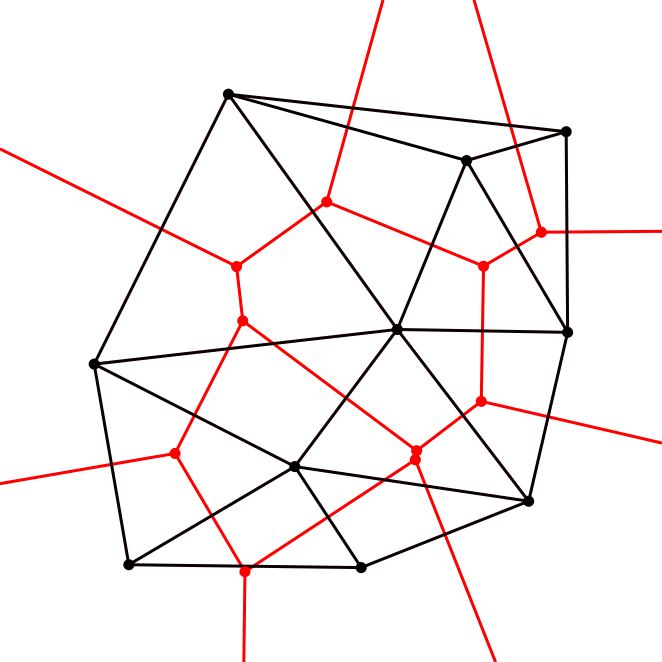
\includegraphics[width=0.6\textwidth]{kuvat/voronoi.png}
  \caption{Mustien pisteiden Delaunayn kolmiointi (mustat viivat) ja sitä vastaava Voronoin tesselaatio punaisella. Punaiset pisteet ovat Delaunayn kolmioinnissa käytettyjen ympyröiden keskipisteitä. (Kuva: Wikimedia Commons -käyttäjä \textit{Hferee}, CC BY-SA 3.0)}
  \label{voronoi}
\end{figure}

Menetelmä on yleistettävissä myös korkeampiin ulottuvuuksiin, jolloin esimerkiksi kolmiulotteisessa tapauksessa syntyy ympyröiden sisällä olevien kolmioiden sijaan pallojen sisällä olevia tetraedrejä. \cite{maur2002delaunay}

\subsection{Algoritmit}

\subsubsection{Kolmiulotteiset algoritmit}

\subsubsection{Quickhull}

\section{Pisteiden generointi ellipsoidin pinnalle}
Jotkin ongelmat vaativat tutkittavan kappaleen pinnan mallintamista pistejoukkona. Tämä on helppo ensiaskel esimerkiksi kappaleen muodon kolmioinnissa. Tässä työssä keskitytään generointimenetelmiin, joita voidaan hyödyntää ellipsoidien mallinnuksessa.

Pisteiden generointiin käytettävät menetelmät voidaan jakaa karkeasti kahteen luokkaan: systemaattisiin ja satunnaisiin menetelmiin. Kummassakin pyritään yleensä luomaan mahdollisimman tasainen jakauma kappaleen pinnalle. Seuraavissa aliluvuissa esitellään yksi systemaattinen ja yksi satunnainen menetelmä.

\subsection{Pisteiden luominen kerroksittain}
Eräs yksinkertainen tapa luoda ellipsin pinnalle pistejoukko, jossa lähimpien pisteiden etäisyydet pysyvät likimain vakioina, on generoida pisteet ellipsin leveyspiirien suuntaisina kehinä. Ellipsi jaetaan $k$ kerrokseen, jolloin navalla olevaan ensimmäiseen ''kerrokseen'' tulee yksi piste, seuraavaan kerrokseen 4 ja tästä kohti päiväntasaajaa kuhunkin kerrokseen aina 4 pistettä enemmän kuin edelliseen. Päiväntasaajan jälkeen pisteiden määrä alkaa jälleen vähentyä neljällä pisteellä kerrosta kohti, kunnes vastakkaisella navalla on jälleen vain yksi piste.

Tämä on yksinkertaisinta tehdä $(\theta, \phi, r)$-koordinaatistossa, jossa $\theta$ mittaa kulmaa navalta kohti päiväntasaajaa ja $\phi$ kulmaa x-akselista positiiviseen kiertosuuntaan z-akselin ympäri. Tällä tavoin generoitaessa kunkin rivin kulmaetäisyydeksi $\theta$-suunnassa muodostuu $\pi/k$ ja kahden saman latitudin pisteen välinen etäisyys $\phi$-suunnassa on $\frac{\pi}{2(k-1)}$.

Näistä pisteistä on yksinkertaista muodostaa ellipsin pinnan kattava kolmiointi, jossa napa toimii kärkenä neljälle kolmiolle ja seuraavan rivin pisteet kussakin oktantissa yhdistävät janat kolmioiden kantoina. Seuraavalla kolmiorivillä edellisen kolmiorivin kantoja vastaa aina kärki ja kunkin oktantin reunoihin muodostuu kaksi uutta kolmiota. Näin jatketaan jälleen päiväntasaajalle asti, minkä jälkeen kolmiot alkavat jälleen vähentyä napaa lähestyttäessä. Kuva 200 kerrosta sisältävästä näin luodusta pistejoukosta on nähtävillä kuvassa \ref{murrikolmiointi}.

\begin{figure}
  \centering
  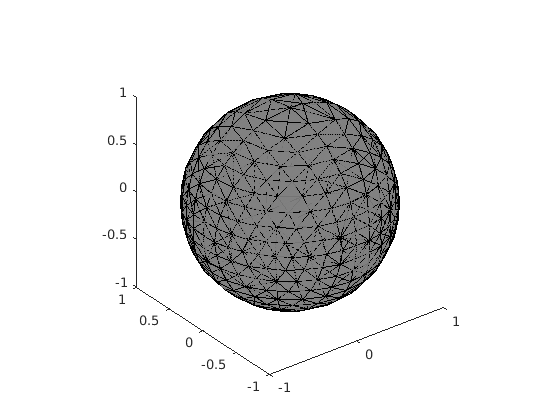
\includegraphics[width=0.6\textwidth]{../Delaunay/data/murrikolmiot/pallo.png}
  \caption{Matlabin \texttt{delanayn}-komentoa käyttäen luotu kuva kerroksittain luodusta pistejoukosta ykikköpallon pinnalla.}
  \label{murrikolmiointi}
\end{figure}

\subsection{Pisteiden arpominen}
Pisteiden generointi satunnaisesti on hyvin yksinkertainen tapa generoida vähällä vaivalla halutunkokoinen pistejoukko. Pallopinnalle generointi on erittäin yksinkertaista. Kun tiedetään haluttu pallon säde, voidaan generoida satunnaisluvut $\theta \in [0, \pi]$ ja $\phi \in [0, 2\pi]$, jolloin saadaan suoraan piste $(\theta, \phi, r)$ missä $r$ on vakio. Esimerkki näin saadusta pistejoukosta on nähtävillä kuvassa \ref{satunnaispallo}.

\begin{figure}[h]
  \centering
  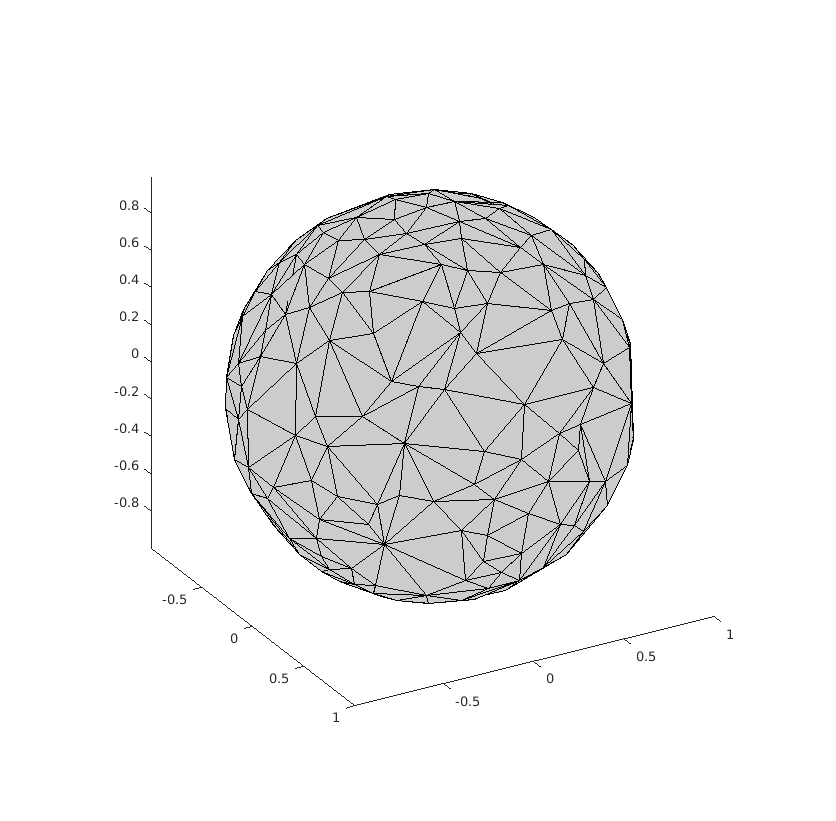
\includegraphics[width=0.8\textwidth]{../Delaunay/data/pallo250/pallo2.png}
  \caption{Yksikköpallon pinnalle satunnaisgeneroitu pistejoukkoon tehty Delaunayn kolmiointi. Pallo koostuu 250 pisteestä ja 505 niiden välille piirretystä kolmiosta.}
  \label{satunnaispallo}
\end{figure}

Ellipsoidin pinnalle generoiminen on kuitenkin monimutkaisempaa, sillä edellä kuvatulla tavalla pistejakaumasta tulee ellipsoidin eksentrisyydestä riippuen mahdollisesti hyvinkin epätasainen. Pohjimmiltaan voidaan kuitenkin käyttää samantyyppistä menetelmää kuin edellä, eli aloittaa generoimalla vastaavat kulmat $\theta$ ja $\phi$ ja määrittämällä näiden perusteella kyseisen pinnan kohdan etäisyys origosta kaavan \ref{r} perusteella, missä $a$, $b$ ja $c$ ovat ellipsin muodon määräävät parametrit ellipsin yhtälöstä (yhtälö \ref{ellipsin-yhtalo}).

\begin{equation}\label{r}
	r(\theta,\phi) = \frac{abc}{\sqrt{b^2c^2\sin^2(\phi)\cos^2(\theta)+a^2c^2\sin^2(\phi)\sin^2(\theta)+a^2b^2cos^2(\phi)}}
\end{equation}

\begin{equation}\label{ellipsin-yhtalo}
	\frac{x^2}{a^2}+\frac{y^2}{b^2}+\frac{z^2}{c^2} = 1
\end{equation}

Eräs tapa huolehtia jakauman tasaisuudesta halutulla tarkkuudella on asettaa tietty kynnysarvo kunkin pisteen ympärillä olevalle säteelle, jonka sisälle ei generoida uusia pisteitä. Tämä voidaan toteuttaa esimerkiksi jakamalla ellipsin pinta-ala halutulla pistemäärällä ja määrittämällä tätä alaa vastaavan ympyrän säde, jolloin voidaan hylätä tätä sädettä lähempänä toista pistettä olevat pisteet. Uusia pisteitä arvotaan, kunnes hyväksyttyjen pisteiden kokonaismäärä on haluttu pistemäärä.

Tätä menetelmää voidaan edelleen kehittää määrittämällä tasaisuuskerroin, jolla kerrotaan saatu ala kutakin pistettä kohden. Pienillä kertoimilla pisteet voivat olla lähempänä toisiaan, jolloin pisteitä hylätään vähemmän eli generointi on nopeampaa, mutta jakauman tasaisuus kärsii. Liian suuren kertoimen valitseminen saattaa johtaa tilanteeseen, jossa uusien kaikki ehdot täyttävien pisteiden generointi on mahdotonta. Esimerkki ellipsoidin pinnalle generoiduista pisteistä on nähtävillä kuvassa \ref{satunnaisellipsoidi}.

\begin{figure}
  \centering
  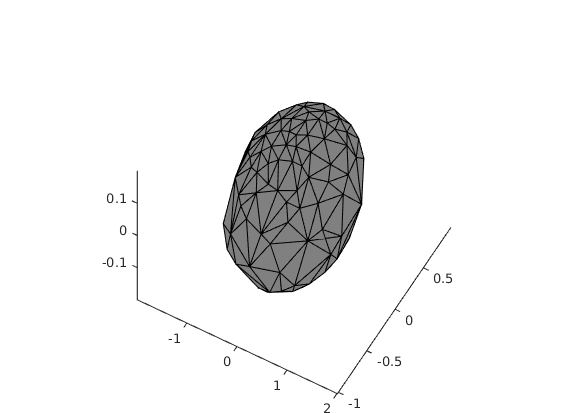
\includegraphics[width=0.8\textwidth]{../Delaunay/data/ellipsoidi150/ellipsoidi.png}
  \caption{Satunnaisgeneroidun pistejoukon Delaunayn kolmiointi ellipsin (a=1,1; b=0,8; c=0,2) pinnalla. Ellipsoidi koostuu 150 pisteestä ja 296 niiden välille piirretystä kolmiosta. Käytetty tasaisuuskerroin on 1,2.}
  \label{satunnaisellipsoidi}
\end{figure}

\section{Lommel-Seeliger -heijastuslaki}
Lommel-Seeliger -heijastuslaki käsittelee yksinkertaista heijastusta, joka tapahtuu puoliäärettömässä väliaineessa, johon valo penetroituu heikentyen absorption ja sironnan vaikutuksesta. Sirottuminen kustakin väliainekerroksesta on isotrooppista ja pintaa kohti sironnut valo heikkenee edelleen matkalla pintaan. \cite{lommel}

Tällöin heijastuskertoimeksi saadaan
\begin{equation}
	\frac{1}{4}\widetilde{\omega}P_{11}(\alpha)\frac{1}{\cos(\epsilon)+\cos(\iota)},
\end{equation}
missä $\epsilon$ on havaitsijan suunnan ja heijastavan pinnan normaalin välinen kulma ja $\iota$ on valonlähteen suunnan ja heijastavan pinnan normaalin välinen kulma. \cite{tenttimatsku, lommel}.

\section{Asteroidin muodon kolmiointi}


\section{Asteroidin sisäinen rakenne}
Kun asteroidin pinta on kolmioitu, voidaan asteroidin sisärakenne kattaa tetraedreillä yksinkertaisesti käyttämällä kutakin kolmiota yhden tetraedrin pohjana ja ellipsoidin keskipistettä tetraedrin neljäntenä kärkenä. Paikkaresoluution parantamiseksi voidaan nämä tetraedrit edelleen jakaa ellipsoidin säteen suunnassa katkaistuihin kartioihin.

Yksinkertaisinta on tehdä jako siten, että kunkin katkaistun kartion korkeus on sama. Tällöin kuitenkin monitahokkaiden tilavuus vaihtelee säteen suunnassa: lähellä keskipistettä tilavuudet ovat pieniä ja lähellä pintaa hyvin suuria. Tästä syystä monissa sovelluskohteissa on hyödyllisempää suunnitella jako monitahokkaisiin siten, että niiden tilavuudet pysyvät likimain samoina.

Tällöin kunkin katkaistun kartion korkeuden laskeminen onnistuu, kun tunnetaan lausekkeet kartion tilavuudelle
\begin{equation}
	V=\frac{1}{3}Ah
\end{equation}
missä $A$ on kartion pohjan ala ja $h$ kartion korkeus, sekä katkaistun kartion tilavuudelle
\begin{equation}\label{katkaistukartio}
	 V = \frac{1}{3} h (A + \sqrt {AA'} + A')
\end{equation}
missä $A$ ja $A'$ ovat pohjien alat ja $h$ on pohjien välinen kohtisuora etäisyys. \cite{wiki:kartio}

Lisäksi tiedetään, että eri katkaistujen kartioiden pohjat ovat yhdenmuotoisia ja niiden alat ovat verrannollisia ellipsoidin keskipisteestä mitatun etäisyyden neliöön. Kun nyt merkitään ellipsoidin sädettä tarkasteltavan tetraedrin kohdalla $R$ (oletetaan, että kolmiot ovat säteeseen verrattuna pieniä, jolloin matka kustakin pohjan pisteestä keskipisteeseen on likimain sama) ja katkaistun kartion korkeutta $h$, saadaan katkaistun kartion pohjien alojen suhteeksi
\begin{equation*}
	A_1=\left(\frac{R-h}{R}\right)^2A_0.
\end{equation*}

Jos kartio halutaan jakaa $n$ osaan, voidaan yhden osan tilavuus laskea yksinkertaisesti
\begin{align}
	V_{katkaistu} &= \frac{1}{n}V_{kokonainen}\nonumber\\
	&= \frac{1}{n}\frac{1}{3}Ah \nonumber
\end{align}
Asetetaan yhtälössä \ref{katkaistukartio} esitetyn katkaistun kartion tilavuus yhtäsuureksi tämän lausekkeen kanssa, jolloin tiedetään
\begin{align}\label{katkaistunkorkeus}
	\frac{1}{3} h (A + \sqrt {AA'} + A') &= \frac{1}{n}\frac{1}{3}Ah &\bigg\vert~ A'=\left(\frac{R-h}{R}\right)^2A \nonumber\\
	h \left(A + \sqrt {A^2\left(\frac{R-h}{R}\right)^2} + \left(\frac{R-h}{R}\right)^2A\right) &= \frac{1}{n}Ah & \nonumber\\
	A\left(1 + \frac{R-h}{R} + \left(\frac{R-h}{R}\right)^2\right) &= \frac{1}{n}A &\nonumber\\
	1 + \frac{R-h}{R} + \left(\frac{R-h}{R}\right)^2 &= \frac{1}{n} &\nonumber\\
	1 + 1-\frac{h}{R} + \left(1-\frac{h}{R}\right)^2 &= \frac{1}{n} &\nonumber\\
	1 + 1-\frac{h}{R} + 1-2\frac{h}{R}+\left(\frac{h}{R}\right)^2 &= \frac{1}{n} &\nonumber\\
	3 - 3\frac{h}{R} +\left(\frac{h}{R}\right)^2 &= \frac{1}{n} &
\end{align}
Yhtälö \ref{katkaistunkorkeus} on yksinkertainen toisen asteen yhtälö, jonka ratkaisuna saadaan $h$:lle seuraava lauseke
	
\section{Asteroidin integroitu kirkkaus}



%%%%% Sisältö loppuu, lähdeluettelo %%%%%
\bibliographystyle{plain}
\bibliography{lahteet} %lähdeluettelon tiedot tiedostossa selkkarilahteet.bib. Esimerkiksi helkasta saa kirjojen tiedot valmiiksi bibtex-muodossa, kannattaa hyödyntää.

\appendix
\newpage
\section{Liittyvä liite.} \label{koodi}
Liian laaja leipätekstiin.
\end{document}
